\chapter{Związek z dominowaniem w grafach}

\section{Definicje: dominowanie i dominowanie rzymskie}
\noindent Niech $G=(V,E)$ będzie grafem prostym.
\begin{description}
  \item[Zbiór dominujący (MDS)] Zbiór $D\subseteq V$ jest dominujący, gdy $\forall v\in V:\ v\in D$ lub $\exists u\in D:\ \{u,v\}\in E$. Celem w problemie MDS jest minimizacja $|D|$.
  \item[Dominacja rzymska (RD)] Funkcja $f:V\to\{0,1,2\}$ jest funkcją dominacji rzymskiej, jeśli każdy wierzchołek z $f(v)=0$ ma sąsiada $u$ z $f(u)=2$. Koszt to $\sum_{v\in V} f(v)$. Celem jest minimizacja kosztu \cite{Cockayne2004,henning2013roman}.
\end{description}

\section{Powiązanie z naszym modelem}
\noindent Model z rozdz.\,2 (\S\ref{sec:model-formal}) ogólnia RD poprzez ograniczenia pojemności grup i rodzinę licencji $\mathcal{L}$. W szczególności:
\begin{theorem}
Jeśli ograniczymy model do dwóch typów: indywidualnej ($c_1=1, m_1=k_1=1$) i „rzymskiej” ($c_g=2, m_g=1, k_g=\infty$), to minimalizacja $\cost(f)$ jest równoważna problemowi RD.
\end{theorem}
\begin{proof}[Szkic]
Ustawienie $c_g=2$ odpowiada wadze $2$ w RD, a $c_1=1$ — wartości $1$. Brak ograniczeń pojemności ($k_g=\infty$) pozwala wierzchołkowi z etykietą 2 „pokrywać” dowolnie wielu sąsiadów $0$, a etykieta $1$ pokrywa jedynie siebie. Mapowanie etykiet $\{0,1,2\}$ na role (R/I/G) i odwrotnie jest obustronnie jednoznaczne i zachowuje koszt, więc optymalne rozwiązania pokrywają się.
\end{proof}

\section{Złożoność i aproksymacje}
\noindent MDS jest NP-zupełny i APX-trudny nawet na grafach o ograniczonym stopniu \cite{ALIMONTI2000123,chlebik2008}. Dominacja rzymska jest NP-trudna \cite{chambers2009} i dla wielu klas dziedziczy ograniczenia aproksymacyjne \cite{POUREIDI2023106363}. Ponieważ nasz model ogólnia RD (dodając limity pojemności), jest co najmniej tak trudny jak RD.

Greedy w stylu pokrycia zbiorów (Set Cover) daje standardowo aproksymację $O(\log n)$ dla MDS i pokrewnych wariantów; przegląd takich wyników można znaleźć m.in. w materiałach wykładowych \cite{Kuhn2012NetworkAlgorithms}.

% \section{Dominowanie w grafach - definicje podstawowe}

% Dominowanie jest jednym z klasycznych zagadnień w teorii grafów, które polega na znalezieniu minimalnego zbioru wierzchołków, które „pokrywają” (dominują) wszystkie inne wierzchołki w grafie. Dokładniej, zbiór dominujący \(D\subseteq V\) w grafie \(G=(V,E)\) to taki zbiór, że każdy wierzchołek \( v \in V \) albo należy do zbioru dominującego, albo ma przynajmniej jednego sąsiada z tego zbioru.

% Formalnie, zbiór \(D \subseteq V\) jest dominujący, jeśli:

% \[
% \forall u \in V: u \in D \lor \exists v \in D : (u, v) \in E
% \]

% Problem znalezienia minimalnego dominowania (\textit{Minimum Dominating Set}) jest klasycznym przykładem problemu NP-trudnego.

% \section{Dominowanie rzymskie - definicja i własności}

% Dominowanie rzymskie jest rozszerzeniem klasycznego dominowania, gdzie każdy wierzchołek przyjmuje jedną z trzech wartości: \(0, 1, 2\). Wierzchołki o wartości \(2\) dominują siebie oraz dowolną liczbę sąsiadów z wartością \(0\), a wierzchołki z wartością \(1\) dominują wyłącznie siebie. Rozwiązanie optymalne minimalizuje sumę wartości przypisanych wierzchołkom:

% \[
% \sum_{v \in V} f(v) \quad \text{(gdzie } f(v) \in \{0,1,2\})
% \]

% Problem ten znany jest jako \textit{Roman domination problem} i jest NP-trudny.

% \section{Dominowanie rzymskie w kontekście modelowania licencji}

% W kontekście optymalizacji zakupu licencji w sieciach społecznościowych można wskazać podobieństwa oraz kluczowe różnice względem problemu dominowania rzymskiego:

% \begin{itemize}
%     \item Wierzchołek o wartości \(2\) (license holder) odpowiada osobie posiadającej licencję grupową, która dominuje siebie oraz sąsiadów należących do grupy.
%     \item Wierzchołek o wartości \(1\) to osoba posiadająca licencję indywidualną.
%     \item Wierzchołek o wartości \(0\) to osoba, która nie posiada własnej licencji, lecz należy do grupy zakupowej sąsiada (license holdera o wartości \(2\)).
% \end{itemize}

% Jednakże występują tutaj istotne różnice:

% \begin{itemize}
%     \item \textbf{Ograniczenie liczby sąsiadów dominowanych}: W dominowaniu rzymskim brak jest ograniczenia liczby sąsiadów dominowanych przez jeden wierzchołek. W naszym modelu licencja grupowa może obejmować tylko od 2 do 6 osób (wliczając posiadacza).
%     \item \textbf{Koszty licencji}: Dominowanie rzymskie ma wartości 0, 1 lub 2 bezpośrednio reprezentujące koszty. W analizowanym modelu koszt licencji grupowej nie jest proporcjonalny do liczby osób, lecz wynosi ok. 2,08-krotność kosztu indywidualnego. Powoduje to dodatkową komplikację przy optymalizacji.
%     \item \textbf{Wymóg sąsiedztwa}: Każdy użytkownik bez własnej licencji musi być bezpośrednim sąsiadem użytkownika posiadającego licencję grupową, co zawęża możliwości tworzenia grup.
% \end{itemize}

% \section{Trudność obliczeniowa problemu}

% Ze względu na powyższe ograniczenia problem optymalizacji zakupu licencji w grafach społecznościowych jest bardziej złożony niż klasyczne problemy dominowania czy dominowania rzymskiego. W istocie jest on uogólnieniem problemów NP-trudnych, ponieważ:

% \begin{itemize}
%     \item W klasycznym dominowaniu liczba sąsiadów dominowanych przez jeden wierzchołek nie jest ograniczona.
%     \item W naszym przypadku musimy dodatkowo brać pod uwagę zarówno ograniczenie na liczbę użytkowników w grupie, jak i specyficzny koszt licencji grupowej w stosunku do indywidualnej.
% \end{itemize}

% W efekcie, przedstawiony problem można uznać za uogólnienie dominowania rzymskiego, co implikuje, że sam również jest NP-trudny. W praktyce oznacza to, że dla dużych grafów nie istnieją znane efektywne algorytmy o wielomianowej złożoności obliczeniowej umożliwiające znalezienie optymalnego rozwiązania w rozsądnym czasie. W związku z tym konieczne jest stosowanie metod heurystycznych lub metaheurystycznych, które dostarczają rozwiązań przybliżonych.

% \section{Podsumowanie}

% Przedstawiony w niniejszym rozdziale model grafowy jest rozszerzeniem klasycznych problemów dominowania, zwłaszcza dominowania rzymskiego. Wskazano na jego specyficzne cechy i ograniczenia wynikające z praktycznych aspektów zakupu licencji oprogramowania w społecznościach. Problemy te są NP-trudne, co uzasadnia konieczność opracowania odpowiednich metod algorytmicznych umożliwiających znalezienie rozwiązań optymalnych lub bliskich optymalnym w akceptowalnym czasie obliczeniowym.

% \section{Podsumowanie rozdziału}

% W tym rozdziale przedstawiony został szczegółowy opis grafowego modelu problemu optymalizacji zakupu licencji oraz jego związek z klasycznym dominowaniem rzymskim. Wyraźnie zaznaczone zostały różnice, które stanowią o unikalności i trudności analizowanego problemu. Na podstawie zdefiniowanego modelu możliwe będzie przeprowadzenie dalszych analiz oraz implementacja różnych algorytmów optymalizacyjnych opisanych w kolejnych rozdziałach pracy.

% TUTAJ WSZYSTKO DO ZREDAGOWANIA
\section{Dominowanie - podstawowe definicje}
% Problematyka dominowania w grafach jest dobrze znana i bogato opisana w literaturze grafowej (zob. np. monografię Haynes i in., 1998 (Dominating set - Wikipedia)). Przypomnijmy podstawowe definicje. Zbiór dominujący w grafie $G=(V,E)$ to taki podzbiór wierzchołków $D \subseteq V$, że każdy wierzchołek spoza tego zbioru ma przynajmniej jednego sąsiada w $D$ (Dominating set - Wikipedia). Innymi słowy, $D$ „dominuje” pozostałe wierzchołki - każdy wierzchołek $v \in V \setminus D$ sąsiaduje z pewnym $u \in D$. Warunek ten można interpretować jako pokrycie wszystkich wierzchołków grafu (poza $D$) przez sąsiedztwa wierzchołków z $D$. Wielkość najmniejszego zbioru dominującego w grafie $G$ nazywamy liczbą dominowania i oznaczamy $\gamma(G)$. Formalnie, $\gamma(G) = \min{|D|: D \subseteq V \text{ jest zbiorem dominującym w } G}$ (Dominating set - Wikipedia). Przykładowo, na rysunku poniżej (graf z wierzchołkami zaznaczonymi kolorem białym) zbiory zaznaczone kolorem czerwonym reprezentują różne dominujące podzbiory: od większego (a) po minimalne (b) i (c). Minimalna liczba dominowania dla tego grafu wynosi 2, co ilustrują przypadki (b) i (c) (Dominating set - Wikipedia).
% (image) Rys. 1: Przykładowe zbiory dominujące (czerwone) w pewnym grafie. (a) Zbiór dominujący o rozmiarze 3 (niemimalny); (b) i (c) przykłady minimalnych zbiorów dominujących o rozmiarze 2, równych $\gamma(G)=2$. Każdy wierzchołek nieczerwony ma sąsiada czerwonego. (Dominating set - Wikipedia)
% Z punktu widzenia naszego problemu, intuicja związana z dominowaniem jest następująca: jeśli potraktujemy osoby posiadające licencje jako zbiór $D$, to warunek, by każdy inny użytkownik miał znajomego z $D$, jest dokładnie warunkiem, by $D$ zapewniał dostęp wszystkim pozostałym (poprzez współdzielenie w ramach krawędzi grafu). Gdybyśmy pominęli rozróżnienie na typy licencji (indywidualna vs. grupowa) i pozwolili każdemu kupującemu obsłużyć wszystkich swoich sąsiadów, wówczas problem minimalizacji kosztu sprowadzałby się wprost do znalezienia minimalnego zbioru dominującego - najmniejszej grupy osób, które wykupią licencje tak, aby cała sieć miała dostęp. W praktyce jednak musimy uwzględnić koszty i ograniczenia, które sprawiają, że sprawa jest bardziej złożona (temu poświęcony będzie rozdz. 3.2 i 3.3). Niemniej jednak, pojęcie dominacji daje pierwszy wgląd w strukturę rozwiązania: jakie osoby pełnią rolę „liderów” zapewniających pokrycie sieci.

Problematyka dominowania w grafach jest dobrze zbadana i szeroko opisana w literaturze~\cite{haynes1998domination}.
Niech \(G = (V,E)\) będzie grafem nieskierowanym.
Zbiorem dominującym nazywamy podzbiór wierzchołków \(D \subseteq V\) taki, że każdy
wierzchołek spoza \(D\) ma co najmniej jednego sąsiada w~\(D\), tj. \[\forall v \in V \setminus D \quad \exists\,u \in D : \{u,v\} \in E.\]
Minimalną liczność zbioru dominującego oznaczamy symbolem \(\gamma(G)\) i nazywamy liczbą dominowania:
\[
\gamma(G) \;=\; \min\bigl\{|D| : D\subseteq V,\; D \text{ jest zbiorem dominującym w } G\bigr\}.
\]

Z punktu widzenia rozważanego problemu zakupu licencji, podstawowe założenie jest następujące:
jeśli potraktujemy osoby kupujące licencje jako zbiór \(D\), a krawędzie grafu jako relacje
umożliwiające udostępnianie licencji, wówczas warunek dominowania opisuje sytuację, w której
każdy użytkownik spoza \(D\) ma znajomego z~\(D\), a zatem uzyskuje dostęp do usługi.
Gdyby wszystkie licencje były identyczne i pozwalały obsłużyć dowolną liczbę sąsiadów,
minimalizacja kosztu sprowadzałaby się do wyznaczenia \(\gamma(G)\).
W praktyce jednak występują różne typy licencji (indywidualne i grupowe) oraz limity
współużytkowników, co czyni problem znacznie bardziej złożonym.

% Minimalny zbiór dominujący nie jest w~ogólności jednoznaczny - graf może mieć wiele
% różnych zbiorów o rozmiarze $\gamma(G)$ co widać na Rysunku \ref{fig:dominatingexample}.
% Decyzyjna wersja problemu („czy w~grafie istnieje zbiór dominujący mocy
% co najwyżej~$k$?”) jest NP-zupełna \cite{karp1972,garey1979}, co sugeruje brak
% algorytmu wielomianowego dla grafu ogólnego.

Należy zauważyć, że minimalny zbiór dominujący nie musi być jednoznaczny. Często bywa tak, że graf ma wiele różnych zbiorów dominujących o rozmiarze równym $\gamma(G)$ (jak na Rys.~\ref{fig:dominatingexample}, gdzie dwa różne zbiory czerwonych wierzchołków są minimalne). Problem znajdowania $\gamma(G)$ jest jednak dobrze określony i należy do klasy problemów NP-trudnych. Jego wersja decyzyjna sformułowana jest następująco: dla zadanego grafu $G$ oraz liczby całkowitej $k$ pytamy, czy istnieje zbiór dominujący o rozmiarze co najwyżej $k$. Jest to klasyczny problem NP-zupełny \cite{wikiDominatingSet, POUREIDI2023106363, PANDA2023337}. Oznacza to, że najprawdopodobniej (przy założeniu $P \neq NP$) nie istnieje algorytm wielomianowy rozwiązujący ten problem w ogólności. W praktyce stosuje się zatem algorytmy przybliżone lub ogranicza analizę do specjalnych klas grafów, dla których problem staje się prostszy. Znane są między innymi efektywne algorytmy zachłanne, które zapewniają rozwiązanie przybliżone z gwarantowanym współczynnikiem. Przykładem jest prosty algorytm zachłanny wybierający kolejno dominujące wierzchołki, osiągający przybliżenie rzędu $O(\ln n)$.


\begin{figure}[ht]
  \centering
  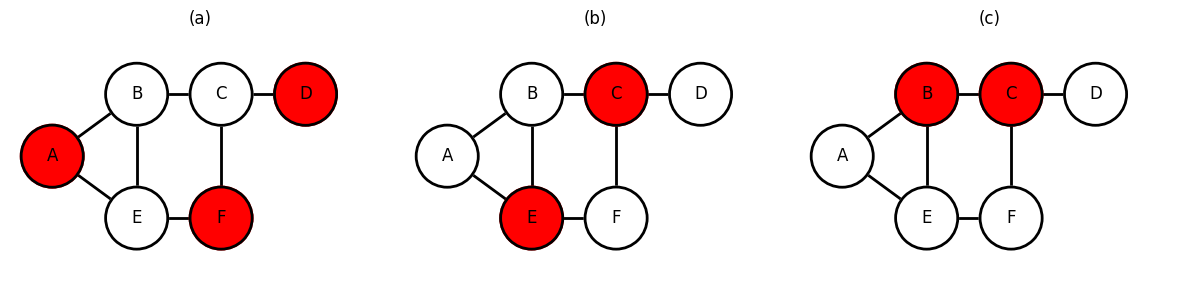
\includegraphics[width=1\textwidth]{assets/dominating-set-example.png}
  \caption[Przykładowe zbiory dominujące]{%
    Przykładowe zbiory dominujące (wyróżnione na czerwono).
    \textbf{(a)}~Zbiór dominujący o mocy~3 .
    \textbf{(b)}-\textbf{(c)}~Dwa różne minimalne zbiory dominujące o mocy~2, zatem
    \(\gamma(G)=2\).  Każdy wierzchołek nieczerwony ma sąsiada czerwonego.
  }
  \label{fig:dominatingexample}
\end{figure}

 \newpage
 Wiadomo jednak, że nie da się w ogólności przekroczyć bariery logarytmicznej. Problem zbioru dominującego jest APX-trudny, a dokładniej log-APX-zupełny \cite{POUREIDI2023106363}. Co więcej, nawet na bardzo ograniczonych grafach, np. grafach o maksymalnym stopniu 3 (grafy kubiczne), problem pozostaje NP-trudny i APX-zupełny \cite{ALIMONTI2000123}. Berman i Fujito (1999) wykazali m.in. NP-trudność pewnych wariantów dominacji w grafach o ograniczonym stopniu \cite{BermanFujitoThreeDegree}, co potwierdza, że zasadnicza trudność problemu dominowania jest obecna już w stosunkowo prostych strukturach.


\section{Dominowanie rzymskie a licencje grupowe}
% Dominowanie rzymskie to wariant problemu dominacji, w którym każdemu wierzchołkowi przypisuje się wartość 0, 1 lub 2. Wierzchołek o wartości 1 pokrywa wyłącznie samego siebie, natomiast wierzchołek o wartości 2 pokrywa siebie oraz wszystkich swoich sąsiadów. Wymaga się, aby każdy wierzchołek o wartości 0 był pokryty przez co najmniej jednego sąsiada o wartości 2. Formalnie, funkcja dominowania rzymskiego na grafie $G=(V,E)$ to funkcja $f: V \to {0,1,2}$ spełniająca warunek, że dla każdego wierzchołka $v$ z $f(v) = 0$ istnieje co najmniej jeden jego sąsiad $u \in V$ taki, że $f(u) = 2$ \cite{Favaron2009}. Wierzchołki z etykietą 2 pełnią rolę „silnych dominatorów”, którzy dominują zarówno siebie, jak i sąsiadów - można je porównać do wierzchołków umieszczających dwie jednostki obrony: jedną chroniącą ich samych i jedną zdolną zabezpieczyć sąsiada. Wierzchołki z etykietą 1 dominują wyłącznie siebie (odpowiednik pojedynczej jednostki obrony niewystarczającej, by ochronić kogoś innego), zaś etykieta 0 oznacza brak dominacji (wymagający ochrony z zewnątrz). Terminologia nawiązuje do legendy o obronie imperium rzymskiego - stąd nazwa; pojęcie to zostało wprowadzone w teorii grafów przez Cockayne’a i współpracowników w 2004 roku \cite{Cockayne2004}.

Dominowanie rzymskie to wariant problemu dominacji, w którym każdemu wierzchołkowi przypisuje się jedną z trzech wartości: 0, 1 lub 2. Wierzchołek o wartości 1 pokrywa wyłącznie samego siebie, natomiast wierzchołek o wartości 2 pokrywa zarówno siebie, jak i wszystkich swoich sąsiadów. Wymaga się przy tym, aby każdy wierzchołek o wartości 0 był pokryty przez co najmniej jednego sąsiada oznaczonego wartością 2. Formalnie, funkcja dominowania rzymskiego na grafie $G=(V,E)$ to funkcja
\[
f: V \to \{0,1,2\},
\]
spełniająca warunek, że dla każdego wierzchołka $v$ z $f(v) = 0$ istnieje sąsiad $u \in V$ taki, że $f(u) = 2$ \cite{Favaron2009}. Minimalizacja sumy wartości $f(v)$ po wszystkich $v \in V$ prowadzi do zdefiniowania tzw. liczby dominowania rzymskiego grafu, oznaczanej $\gamma_R(G)$.

Terminologia i metafora związana z dominacją rzymską wywodzą się z legendy o obronie granic imperium rzymskiego. Zakładano w niej, że w każdej osadzie można umieścić pewną liczbę jednostek wojskowych. Osada z dwiema jednostkami była w stanie bronić się samodzielnie i jednocześnie wysłać wsparcie do sąsiedniej osady. Lokacja z jedną jednostką potrafiła bronić tylko siebie, a miejscowości pozbawione jednostek militarnych wymagała ochrony z zewnątrz. W tej metaforze graf reprezentuje system osad i połączeń między nimi, a etykiety 0, 1 i 2 odpowiadają decyzjom o rozmieszczeniu wojsk. Koncepcję dominowania rzymskiego wprowadzili do teorii grafów Cockayne i współpracownicy w 2004 roku \cite{Cockayne2004}.

% W kontekście problemu optymalnego zakupu licencji w grafach przedstawiających sieci społecznościowe interpretacja jest następująca: etykieta $f(v)=2$ odpowiada użytkownikowi $v$, który wykupił licencję grupową (przez co zabezpiecza „dostęp” sobie oraz przynajmniej jednemu sąsiadowi). Etykieta $f(v)=1$ odpowiada użytkownikowi z licencją indywidualną (zapewniającą dostęp tylko jemu samemu). Natomiast $f(v)=0$ oznacza użytkownika bez własnej licencji, który musi polegać na dostępie od kogoś innego. Warunek dominowania rzymskiego, że każdy $0$ ma sąsiada $2$, gwarantuje dokładnie to, co w naszym modelu jest wymagane - każda osoba bez licencji ma znajomego z licencją grupową, który może się z nią podzielić dostępem. W ten sposób, każda funkcja $f: V \to {0,1,2}$ spełniająca warunki dominowania rzymskiego wyznacza pewną realizację strategii licencyjnej w naszej sieci.

W kontekście problemu optymalnego zakupu licencji w grafach reprezentujących sieci społecznościowe interpretacja jest bezpośrednia. Wartość $f(v)=2$ odpowiada użytkownikowi $v$, który nabywa licencję grupową i zapewnia dostęp zarówno sobie, jak i co najmniej jednemu ze swoich sąsiadów. Wartość $f(v)=1$ oznacza użytkownika posiadającego licencję indywidualną, pokrywającą wyłącznie jego samego. Natomiast $f(v)=0$ reprezentuje użytkownika bez własnej licencji, który musi polegać na pokryciu przez sąsiada z wartością 2. Warunek dominowania rzymskiego, zgodnie z którym każdy wierzchołek z etykietą 0 ma sąsiada z etykietą 2, gwarantuje dokładnie to, co w naszym modelu jest wymagane: każdy użytkownik bez licencji ma znajomego z licencją grupową, który może podzielić się z nim dostępem. W ten sposób każda funkcja $f:V \to \{0,1,2\}$ spełniająca warunki dominowania rzymskiego wyznacza dopuszczalną strategię licencyjną w rozważanej sieci.

% Waga funkcji dominowania rzymskiego definiowana jest jako $w(f) = \sum_{v \in V} f(v)$, czyli suma przypisanych wartości. Liczba dominowania rzymskiego $\gamma_R(G)$ to najmniejsza możliwa waga funkcji dominowania rzymskiego dla grafu $G$. Jeśli przyjmiemy, że koszt licencji indywidualnej wynosi 1, a grupowej to 2, to minimalizacja kosztu w naszym problemie pokrywa się dokładnie z zagadnieniem znalezienia funkcji dominowania rzymskiego o minimalnej wadze. Cel minimalizacji sumarycznego kosztu $C = |I| + 2|G|$ jest zatem identyczny z minimalizacją $w(f)$, gdy utożsamimy $|I|$ z liczbą wierzchołków o etykiecie 1, a $|G|$ - o etykiecie 2. Innymi słowy, dla przypadku $p=2$ problem optymalnego zakupu licencji jest równoważny problemowi dominowania rzymskiego na grafie znajomości.

Waga funkcji dominowania rzymskiego definiowana jest jako $w(f) = \sum_{v \in V} f(v)$, czyli suma przypisanych wartości. Liczba dominowania rzymskiego $\gamma_R(G)$ to najmniejsza możliwa waga funkcji dominowania rzymskiego dla grafu $G$. Jeśli przyjmiemy, że koszt licencji indywidualnej wynosi 1, a grupowej 2, to minimalizacja kosztu w naszym problemie pokrywa się z zagadnieniem znalezienia funkcji dominowania rzymskiego o minimalnej wadze. Cel minimalizacji sumarycznego kosztu
\[
C = |I| + 2|G|
\]
jest zatem równoważny minimalizacji $w(f)$, gdy utożsamimy $|I|$ z liczbą wierzchołków o etykiecie 1, a $|G|$ o etykiecie 2. Należy jednak podkreślić, że pełna równoważność z dominowaniem rzymskim zachodzi tylko wtedy, gdy liczba sąsiadów dowolnego wierzchołka nie przekracza maksymalnej liczby użytkowników dopuszczonych w planie grupowym. Jak wspomniano wcześniej przy omawianiu parametrów $m$ i $k$, nasze ujęcie wprowadza dodatkowe ograniczenie pojemności - wierzchołek o wartości 2 może pokrywać jedynie ograniczoną liczbę sąsiadów. Problem optymalnego zakupu licencji jest więc uogólnieniem dominowania rzymskiego, dostosowanym do praktycznych limitów występujących w planach subskrypcyjnych.

% W przypadku innych modeli cenowych, dominacja rzymska stanowi nadal użyteczną metaforę, choć nie oddaje w sposób wystarczający struktury kosztów. Gdy $p \neq 2$, możemy rozważyć ogólniejsze przypisania wag. Przykładowo w sytuacji, gdy $p=3$, to licencja grupowa ma wartość 3 jednostek kosztu, co nie mieści się w klasycznym schemacie ${0,1,2}$, gdzie 2 jest maksymalną wartością. Istnieją jednak rozszerzenia pojęcia dominowania rzymskiego - np. $k$-dominacja rzymska, gdzie używa się wartości ${0,1,\dots,k}$ \cite{CHAUDHARY2024301}, albo koncepcja dominowania rzymskiego z wagami \cite{Ghaffari2020}. W przypadku $p=3$ można by dopuścić etykietę $3$ oznaczającą specjalny rodzaj wierzchołka ze zbioru dominującego zdolnego ochraniać dwóch sąsiadów, co odpowiadałoby planowi droższemu, ale o większej pojemności. W literaturze pojawiły się uogólnienia pokrewne temu pomysłowi, np. tzw. dominacja podwójnie rzymska i inne warianty.

W przypadku innych modeli cenowych, dominacja rzymska stanowi nadal użyteczną metaforę, choć nie oddaje w sposób wystarczający struktury kosztów. Gdy $p \neq 2$, możemy rozważyć ogólniejsze przypisania wag, w których etykieta odpowiada rzeczywistemu kosztowi planu. Przykładowo, gdy $p=3$, to licencja grupowa ma koszt równy trzem jednostkom, co nie mieści się w klasycznym schemacie $\{0,1,2\}$. W literaturze zaproponowano rozszerzenia pozwalające modelować takie sytuacje, m.in. $k$-dominację rzymską, gdzie dopuszcza się wartości $\{0,1,\dots,k\}$ \cite{CHAUDHARY2024301}, czy też dominację rzymską z wagami \cite{Ghaffari2020}. Warianty te pozwalają odwzorować przypadki, w których dostępne są plany o różnych kosztach i różnej pojemności, np. licencja droższa, ale umożliwiająca współdzielenie w większej grupie. W tym sensie uogólnienia dominowania rzymskiego są bliższe rzeczywistemu problemowi optymalizacji kosztów licencji niż klasyczna wersja ograniczona do wartości 0, 1 i 2.

% Na potrzeby tej pracy nie musimy jednak wchodzić w tak szczegółowe odmiany. Wystarczy stwierdzić, że dominowanie rzymskie bardzo dobrze modeluje sytuację zakupu licencji w przypadku najprostszego i dość reprezentatywnego modelu. W praktyce, jeśli $p$ jest większe, strategia optymalna często i tak polega na wykorzystaniu licencji grupowych do pełnego obsadzenia nimi maksymalnej liczby osób, co czyni opis dominacją rzymską użytecznym do wyznaczenia „kto powinien kupić licencję grupową” (etykiety 2) a kto może pozostać bez zakupu (0) lub ewentualnie kupić licencję indywidualną (1).

Na potrzeby tej pracy nie jest jednak konieczne wchodzenie w szczegółowe odmiany dominowania rzymskiego. Wystarczy zauważyć, że w analizowanym modelu schemat pozostaje taki sam jak w klasycznej wersji, a jedyną różnicą jest koszt przypisywany wierzchołkom o etykiecie $2$. W zależności od przyjętego modelu cenowego wartość ta może wynosić $p=2$, ale równie dobrze $p=1{,}5$ czy $p=3$. Konstrukcja funkcji dominowania rzymskiego oraz sam podział na etykiety $\{0,1,2\}$ nie ulega zmianie. Innymi słowy, dominacja rzymska dostarcza prostego i intuicyjnego opisu sytuacji: etykieta $2$ oznacza użytkownika z licencją grupową, etykieta $1$ - użytkownika z licencją indywidualną, a etykieta $0$ - osobę, która musi korzystać z dostępu od sąsiada.


% Prosty przykład obrazujący wykorzystanie dominowania rzymskiego. Weźmy graf w kształcie gwiazdy: jeden centralny wierzchołek $A$ połączony z kilkoma liśćmi $B,C,D,E$. Intuicyjnie, najlepszą strategią jest, by centralny użytkownik $A$ wykupił licencję grupową, z której skorzystają wszyscy jego sąsiedzi. W naszym modelu odpowiada to przypisaniu $f(A)=2$, zaś dla każdego liścia $X \in {B,C,D,E}$ przypisaniu $f(X)=0$. Warunek dominowania rzymskiego jest spełniony, bo każdy $0$ (np. $B$) ma sąsiada $A$ z $f(A)=2$. Waga takiej funkcji to $w(f) = 2 + 0+0+0+0 = 2$. Rzeczywiście, koszt dla grupy ${A,B,C,D,E}$ wynosi 2 (jedna licencja grupowa). Gdybyśmy zamiast tego wybrali strategię indywidualną dla każdego (wszyscy $f=1$), waga wyniosłaby $5$, a koszt 5. Gdyby centralny kupił licencję indywidualną, a liście pozostałyby bez dostępu, warunek nie byłby spełniony bo liście nie miałyby sąsiada z $2$. Przykład ten przedstawiony jest na Rysunku \ref{fig:romandomatinonstarexamepl} i pokazuje, jak dominacja rzymska wskazuje optymalny wybór „lidera” (centrum gwiazdy) z mocniejszym statusem (2). Oczywiście, w większych grafach może być wielu kandydatów na licencje grupowe - problem ich doboru to właśnie zagadnienie optymalnej dominowania rzymskiego.

Prosty przykład zastosowania dominowania rzymskiego daje graf w kształcie gwiazdy. Centralny wierzchołek $A$ jest połączony z liśćmi $B, C, D, E$. Najlepszą strategią jest, aby $A$ wykupił licencję grupową i udostępnił ją wszystkim swoim sąsiadom. W modelu oznacza to $f(A)=2$, a dla każdego liścia $f(B)=f(C)=f(D)=f(E)=0$. Warunek dominowania rzymskiego jest spełniony, ponieważ każdy liść o wartości 0 ma sąsiada $A$ o wartości 2. Waga funkcji wynosi wówczas $w(f)=2$ - odpowiada to kosztowi jednej licencji grupowej obsługującej całą pięcioosobową grupę.

Dla porównania można rozważyć inne strategie. Jeśli każdy wierzchołek kupiłby licencję indywidualną ($f=1$), waga wyniosłaby $5$ - koszt pięciu osobnych licencji. Jeśli centralny wierzchołek kupiłby tylko licencję indywidualną ($f(A)=1$), a liście pozostałyby bez dostępu, warunek nie byłby spełniony - żaden liść nie miałby sąsiada o wartości 2.

Rysunek~\ref{fig:romandomatinonstarexamepl} ilustruje ten przykład i pokazuje, jak dominowanie rzymskie wskazuje optymalny wybór użytkownika pełniącego rolę lidera w centrum gwiazdy. W większych grafach kandydatów do roli właścicieli licencji grupowych jest więcej - ich odpowiedni dobór prowadzi już do właściwego problemu optymalizacji dominowania rzymskiego.


\begin{figure}[ht]
  \centering
  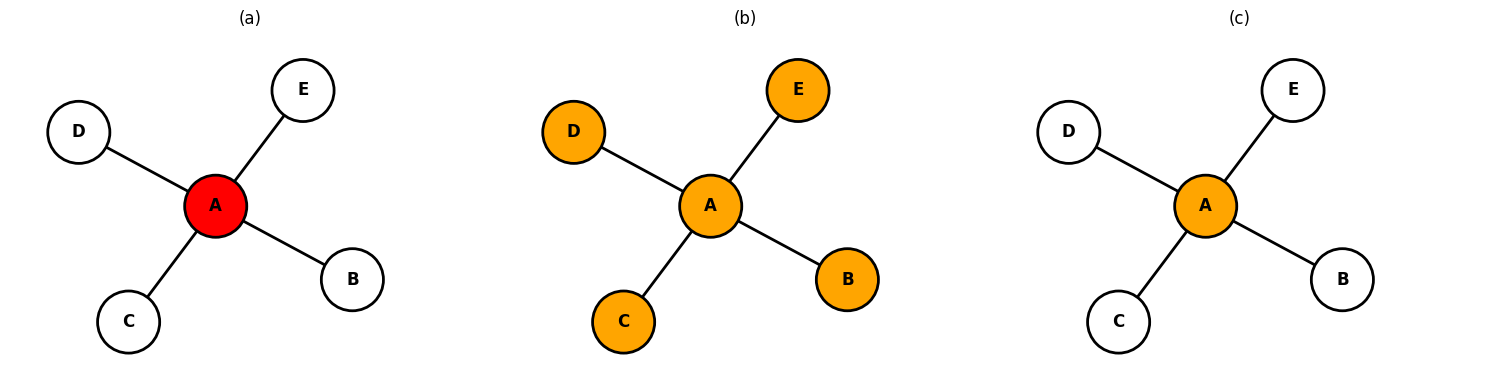
\includegraphics[width=1\textwidth]{assets/stars.png}
  \caption{
    Kolory: biały = $0$, pomarańczowy = $1$, czerwony = $2$.
    \textbf{(a)}~Przypisanie optymalne (koszt 2).
    \textbf{(b)}~Wszyscy z $f=1$ (koszt 5).
    \textbf{(c)}~$A=1$, liście $f=0$ (niespełniony warunek).
  }
  \label{fig:romandomatinonstarexamepl}
\end{figure}


% W interpretacji dominowania rzymskiego warto wspomnieć, że oryginalna inspiracja historyczna zakładała, iż wierzchołek z dwoma oddziałami może w razie potrzeby przenieść jeden oddział do sąsiada pozbawionego obrony. W naszej analogii oznacza to, że osoba z licencją grupową może udostępnić dostęp przynajmniej jednemu znajomemu. Jeśli dany „silny” wierzchołek ma wielu sąsiadów oznaczonych 0, to formalnie warunki dominowania rzymskiego są spełnione. Jednak w interpretacji praktycznej jeden abonament grupowy ma ograniczoną liczbę slotów, więc jeden użytkownik nie może nieograniczenie wielu osobom zapewnić dostępu. Stąd nasz problem jest nieco bardziej ograniczony niż klasyczne dominowanie rzymskie - jeden wierzchołek 2 może „pokryć” co najwyżej $L$ wierzchołków 0 (sąsiadów). Gdy $L$ jest małe, może zajść potrzeba, by niektóre duże gwiazdy w grafie miały więcej niż jeden „silny” wierzchołek. Mimo tego ograniczenia, wiele intuicji z teorii dominowania rzymskiego wciąż obowiązuje przy konstruowaniu rozwiązań - wierzchołki 2 powinny być rozmieszczone tak, by objąć wszystkich 0 w swoim sąsiedztwie, a wierzchołki 1 będą pojawiać się tylko tam, gdzie opłaca się komuś kupić indywidualnie zamiast korzystać od kogoś.

\section{Złożoność obliczeniowa problemu}

% Skoro udało się sprowadzić problem zakupu licencji do problemu dominowania w grafach, można skorzystać z wiedzy o złożoności tego zagadnienia. Niestety, problem ten okazuje się NP-trudny w ogólności. Już klasyczny problem zbioru dominującego jest NP-zupełny (decyzyjnie) \cite{booth1980dominating}, a dominowanie rzymskie również należy do klasy problemów NP-trudnych. Istnieje redukowanie problemu dominowania rzymskiego do dominującego lub odwrotnie dla wielu klas grafów, co wskazuje na zbliżony poziom trudności. Intuicyjnie, dopuszczenie stanów 0,1,2 czyni problem co najmniej tak trudnym jak zwykłe dominowanie - można to sobie wyobrazić, zauważając że jeśli ograniczyć rozwiązania dominowania rzymskiego do takich, gdzie $f(v)$ przyjmuje tylko wartości 0 lub 1, to znajdujemy się w ustawieniu odpowiadającym zwykłemu dominowaniu. Zatem dominacja rzymska ogólna zawiera jako podprzypadek dominację klasyczną, co implikuje NP-trudność. Dokładniejsze dowody złożoności znajdują się w literaturze - np. pokazano NP-zupełność problemu dominowania rzymskiego poprzez redukcję z pokrycia wierzchołków lub zbioru dominującego \cite{chambers2009}. W kontekście naszego problemu oznacza to, że optymalne wyznaczenie, którzy użytkownicy powinni kupić jakie licencje, jest obliczeniowo trudne dla dużych sieci. Mówiąc wprost, nie istnieje znany algorytm, który w czasie wielomianowym znajdzie rozwiązanie minimalnego kosztu dla dowolnej struktury znajomości - trzeba by sprawdzić kombinacje wyborów, co w najgorszym razie rośnie wykładniczo z liczbą wierzchołków.

Sprowadzenie problemu zakupu licencji do problemu dominowania w grafach pozwala odwołać się do znanych wyników o złożoności obliczeniowej. Niestety, problem ten jest w ogólności NP-trudny. Już klasyczny problem zbioru dominującego należy do klasy NP-zupełnych w wersji decyzyjnej \cite{booth1980dominating}, a dominowanie rzymskie również zostało sklasyfikowane jako NP-trudne. Istnieją redukcje pomiędzy tymi problemami dla wielu klas grafów, co wskazuje na ich zbliżony poziom trudności. Intuicyjnie, dopuszczenie etykiet $0,1,2$ czyni problem co najmniej tak trudnym jak klasyczne dominowanie - wystarczy ograniczyć funkcje dominowania rzymskiego do wartości $\{0,1\}$, aby uzyskać zwykły problem zbioru dominującego. W ten sposób dominowanie rzymskie zawiera dominację klasyczną jako szczególny przypadek, co implikuje jego NP-trudność.

Dokładne dowody znajdują się w literaturze - np. pokazano NP-zupełność problemu dominowania rzymskiego poprzez redukcję z problemu pokrycia wierzchołków lub zbioru dominującego \cite{chambers2009}. W kontekście naszego modelu oznacza to, że optymalne wyznaczenie użytkowników kupujących poszczególne licencje jest obliczeniowo trudne dla dużych sieci. Innymi słowy, nie istnieje znany algorytm wielomianowy, który gwarantowałby znalezienie rozwiązania minimalnego kosztu dla dowolnej struktury grafu znajomości - w najgorszym przypadku liczba kombinacji rośnie wykładniczo wraz z liczbą wierzchołków.

Konsekwencją NP-trudności jest także brak prostego schematu aproksymacyjnego dla problemu minimalizacji kosztów licencji. Ponieważ problem dominowania (minimalnego zbioru dominującego) jest APX-zupełny (dla konkretnych rodzajów grafów) \cite{POUREIDI2023106363}, nie ma wielomianowego schematu aproksymacji (PTAS) gwarantującego dobre przybliżenie. Dla naszego problemu, który jest uogólnieniem dominowania, można oczekiwać podobnych ograniczeń - prawdopodobnie nie da się znaleźć w czasie wielomianowym rozwiązań bliższych optimum niż o czynnik $O(\ln n)$ w najgorszym przypadku. Proste heurystyki zachłanne mogą jednak dawać przyzwoite wyniki. Na przykład, heurystyka wybierająca iteracyjnie wierzchołek, który pokrywa najwięcej jeszcze niepokrytych sąsiadów (i dająca mu licencję grupową), jest jedną z implementacji algorytmu zachłannego dla zbioru dominującego i osiąga współczynnik $\approx (2 + \ln \Delta)$, gdzie $\Delta$ to maksymalny stopień grafu \cite{Kuhn2012NetworkAlgorithms}. W najgorszym razie jest to $O(\ln n)$, ale dla wielu grafów rzeczywiste wyniki są lepsze niż ta pesymistyczna granica. Ważnym faktem jest też to, że problem pozostaje trudny nawet dla grafów o niewielkich stopniach - np. wykazano, że dla grafów o stopniu mniejszym bądź równym cztery minimum dominujące jest APX-zupełne \cite{ALIMONTI2000123, POUREIDI2023106363}. To implikuje, że ograniczenie maksymalnej liczby znajomych nie czyni problemu trywialnym. W kontekście subskrypcji oznacza to, że nawet w sieci gdzie każdy zna tylko kilka osób, optymalny dobór kto z kim powinien się połączyć we wspólnej licencji nadal może wymagać złożonych obliczeń.

Biorąc powyższe pod uwagę, w dalszej części badania główny nacisk zostanie położony na podejścia algorytmiczne, które biorą pod uwagę tę złożoność. Ponieważ nie istnieje wydajny algorytm dokładny dla ogólnego przypadku, rozważymy dwutorowo: (a) zastosowanie metod dokładnych dla umiarkowanych rozmiarów oraz (b) zaprojektowanie i analiza algorytmów heurystycznych zdolnych dawać dobre rozwiązania dla większych sieci. W literaturze pojawiły się już pierwsze próby wykorzystania technik optymalizacyjnych do problemu dominacji. Przykładowo, Parra Inza i in. (2022) zaproponowali sformułowanie problemu dominującego jako ILP oraz heurystyki naprawcze dla jego rozwiązywania \cite{PARRAINZA2024926}. Takie podejście można zaadaptować do omawianego problemu, wprowadzając zmienne decyzyjne wskazujące wybór typu licencji dla każdego użytkownika i ograniczenia. Z drugiej strony, heurystyki takie jak algorytm zachłanny, algorytmy lokalnej optymalizacji czy metaheurystyki - np. algorytmy genetyczne, symulowane wyżarzanie - mogą być użyte, by szybko przeszukać przestrzeń możliwych konfiguracji licencji.
